\chapter{Requisiti e casi d'uso}\label{chap:requisiti}
In questo capitolo saranno elencati ed esplicati i requisiti per la realizzazione dell'applicazione e i possibili casi d'uso.

\section{Requisiti}\label{sec:requisiti}
Il funzionamento che si vuole ottenere dall'applicazione è descritto dalla seguente rappresentazione:

\begin{figure}[H]
    \centering
    \resizebox{1.0\textwidth}{!}{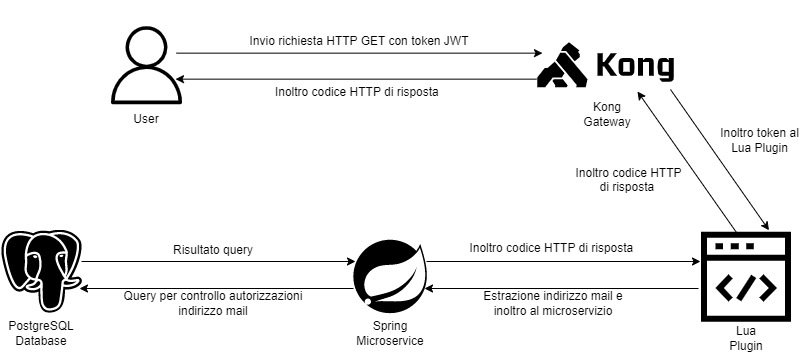
\includegraphics{img/comunicazioni_applicazioni.drawio.png}}
    \caption{Schema comunicazioni}
    \label{fig:comunicationscheme}
\end{figure}

Ricapitolando, dallo schema delle comunicazioni si evince che il funzionamento dell'applicazione si articola in:
\begin{enumerate}
\item Invio della richiesta \texttt{HTTP GET} dall'utente a Kong Gateway;
\item Inoltro del token all'interno della richiesta da Kong Gateway al plugin Lua;
\item Estrapolazione dell'indirizzo mail dal token ricevuto (verificandone anche l'integrità);
\item Richiesta \texttt{HTTP GET} dal plugin al microservizio Spring;
\item Operazioni per il collegamento al Database;
\item Esecuzione della query per verificare le autorizzazioni dell'indirizzo mail ricevuto;
\item Ottenimento del risultato della query;
\item Si rimanda l'informazione ottenuta effettuando il percorso inverso, fino a comunicarla all'utente. 
\end{enumerate}

\section{Casi d'uso}\label{sec:casiuso}
L'applicazione da realizzare risulta adatta per l'integrazione su tutte le piattaforme che offrano dei servizi gratuiti e a pagamento, infatti, lo scopo è quello di 
determinare quali utenti di un'eventuale piattaforma siano autorizzati ad accedere a determinati servizi.\\ \\
Un reale esempio di applicazione del prodotto può essere una piattaforma che fornisca servizi di PEC (Posta Elettronica Certificata) ma anche di fatturazione elettronica.\\
Si supponga che l'utilizzo della PEC sia gratuito per tutti gli utenti registrati, mentre la fatturazione elettronica sia riservata ai soli utenti che abbiano sottoscritto 
un abbonamento: in questo caso il prodotto realizzato soddisferebbe la necessità di controllare a quali livelli della piattaforma un determinato utente ha il permesso di accedere.
